\documentclass[conference]{IEEEtran}
\IEEEoverridecommandlockouts
% The preceding line is only needed to identify funding in the first footnote. If that is unneeded, please comment it out.
\usepackage{cite}
\usepackage{amsmath,amssymb,amsfonts}
\usepackage{algorithmic}
\usepackage{graphicx}
\usepackage{textcomp}
\usepackage{xcolor}
\usepackage{url}
\usepackage{hyperref}
\usepackage{float}
\def\BibTeX{{\rm B\kern-.05em{\sc i\kern-.025em b}\kern-.08em
    T\kern-.1667em\lower.7ex\hbox{E}\kern-.125emX}}
\begin{document}

\title{Dynamic and Stable (DAS) Page Replacement Algorithm\\

\thanks{https://github.com/RamyaDanappa/DAS-page-replacemnt-algorithm}


}

\author{\IEEEauthorblockN{1\textsuperscript{st} Milin Mistry}
\IEEEauthorblockA{\textit{DA-IICT, Gandhinagar} \\
%\textit{Institute of Information & Communication Technology}\\
%Gandhinagar \\
201801125@daiict.ac.in}
\and
\IEEEauthorblockN{2\textsuperscript{nd} Varshit Maisuriya}
\IEEEauthorblockA{\textit{DA-IICT, Gandhinagar} \\
%\textit{Institute of Information & Communication Technology}\\
%Gandhinagar \\
201801455@daiict.ac.in}
\and
\IEEEauthorblockN{3\textsuperscript{rd} Darshil Rana}
\IEEEauthorblockA{\textit{DA-IICT, Gandhinagar} \\
%\textit{Institute of Information & Communication Technology}\\
%Gandhinagar \\
201801462@daiict.ac.in}

}

\maketitle

\begin{abstract}
We implemented a new page replacement policy called Dynamic and Stable (DAS) page replacement policy and compared it with different policies on some standard data-sets/trace files. The algorithm has outperformed some standard cache replacement Algorithms like LRU and LFU. We modified the policy with having adaptivity which resulted in increment of performance to the original algorithm.\\
\\
Github-Repo:
\url{https://github.com/VarshitMaisuriya/DAS-PageReplacementPolicy}
\end{abstract}

%\begin{IEEEkeywords}
%component, formatting, style, styling, insert
%\end{IEEEkeywords}

\section{\textbf{Introduction}}

In an operating system that uses paging for memory management, a page 
replacement algorithm is needed to decide which page needs to be replaced when 
new page comes in. As we know that cache has a finite amount of size so whenever we want to access some page and cache is full then we need to evict some page based on different kinds of algorithms which are known as page replacement algorithms.

Further, the efficiency of the algorithm depends upon the faults encountered and thus the eviction strategy needs to be decided properly.


\section{\textbf{types of page replacement policies}}

Some of the standard page-replacement policies are:
\begin{itemize}
    \item Belady's OPT page replacement policy
    \item FIFO (First In First Out)
    \item LRU (Least Recently Used)
    \item LFU (Least Frequently Used)
\end{itemize}

\section{\textbf{Implementation}}
Following are the page replacement policies which we implemented for testing and comparison purposes. We implemented DAS policy from the research paper we studied and further implemented our proposed change in the policy i.e. Adaptive-DAS and tested them on different traces.

\subsection{\textbf{Belady's OPT page replacement policy}}

The OPT algorithm is a theoretical concept that works as \textit{ "whenever a page needs to be swapped we evict the page which will be used farthest in the future"}. Thus, OPT algorithm provides an upper bound on the achievable hit-ratio for given accesses and cache size.
\\
\subsubsection*{Drawbacks}

\begin{itemize}
    \item It is not practical, as future predictions on the accesses can not be determined.
    \item  It can not be used in real-time applications as it is an offline algorithm.
\end{itemize}

\subsection{\textbf{Least Recently Used (LRU)}}

In this policy , we evict a page which was used furthest in the past. It means that page with the lowest recency will be removed from the cache whenever there is a miss and cache is full.
\\
\subsubsection*{Drawbacks}

\begin{itemize}
    \item It does not perform well in weak localities because it does not consider frequencies.
    \item  LRU does not perform well in sequential access.
    \item There is a problem in loop access because in a loop , element with the least recency has very high probability to be accessed in the future.

\end{itemize}

\subsection{\textbf{Least Frequently Used (LFU)}}

This algorithm computes the frequency of access for every block. When the block 
present in the cache is accessed the block’s frequency will increase, when a block 
not present in the cache is accessed then the newly accessed block replaces the 
least frequency block in the cache.
\\
\subsubsection*{Drawbacks}

\begin{itemize}
    \item This algorithm is frequency-based and ignore recency.
    \item It gives bad performance under temporally clustered type data accesses

\end{itemize}

As we saw that both recency and frequency are important things needed to be considered for better efficiency, we need a new policy that considers both things and thus we have worked on DAS (Dynamic and Stable) Page Replacement Policy that considers both recency and frequency parts of the accesses which is explained below.

\subsection{\textbf{Dynamic and Stable (DAS)}}

General idea in DAS policy is that we divide our cache into 2 part: LRU part and LFU part. Thus, cache have a hybrid-structure.

LRU-portion contains the most recently used blocks i.e. considers recency and  LFU-portion includes the most frequently used blocks i.e. considers frequency. Also, the frequencies of the blocks in LRU-portion will always be less than the minimum frequency of blocks present in LFU-portion. Thus, overall cache acts as partial LRU and partial LFU as shown in figure below.

\begin{figure}
        \centering
       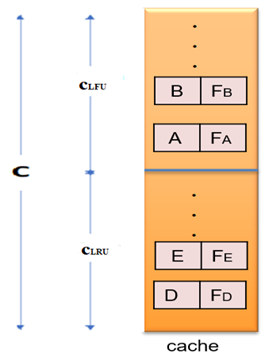
\includegraphics[scale=0.6]{Picture1.png}~
       \caption{DAS - Cache structure}\label{Fig:1}
 \end{figure}
Thus, at any instant:
\begin{equation}
    C_{tot} = C_{LRU} + C_{LFU}
\end{equation}
Here, \\
$C_{tot}$ = Total cache-size \\
$C_{LRU}$ = Cache size of LRU-portion \\
$C_{LFU}$ = Cache size of LFU-portion \\

\\
\\

\subsubsection*{\textbf{Cache-Replacement Policy for DAS}}-

Initially, the cache is empty. For empty cache references, first we will fill the empty portion of LRU, and then we will fill the empty portion of LFU. Now, if the cache is full and we try to access a block say ‘X’, then one the following cases will be performed.\\

\begin{itemize}
    \item \textbf{ Case 1: Block X is present in LFU portion :}
    \begin{itemize}
        \item Considered hit in the cache.
        \item Increment of the frequency of the block X in LFU portion.
    \end{itemize}
    
    \item \textbf{ Case 2: Block X is present in LRU portion :}
    \begin{itemize}
        \item Considered hit in the cache.
        \item Increment of the frequency of the block X in LRU portion.
        \item Now, block X can be moved to LFU portion if one of the two conditions occurs.
        \begin{enumerate}
        
            \item If there is space available in LFU portion then we will add this block in LFU portion.
            \item If the minimum frequency of the block in LFU-portion is less than the frequency of block X, then we will exchange those 2 blocks.

        \end{enumerate}
    \end{itemize}
    
    \item \textbf{ Case 3: Block X is not present in cache :}
    \begin{itemize}
        \item Considered miss in the cache.
        \item We add block X in the LRU portion if it has free space .
        \item If LRU portion is full then we evict the block with the least recency and add block X at the top of the LRU portion and create frequency associated with that block X .

    \end{itemize}
    
\end{itemize}\\

\subsection{\textbf{Adaptive-DAS}}

This algorithm is ours proposed change to the existing DAS policy. The motive of this policy is instead of dynamic, we need to think adaptive. So, the motivation of this algorithm is from ARC Policy (Adaptive Replacement Cache Policy).\\

For adaptive nature, along with the hybrid cache, we use 2 ghost caches, one for LRU and one for LFU portion. These ghost caches keep track of recent eviction history of corresponding cache i.e LRU ghost will store the blocks that are recently evicted from LRU part of original cache and similarly LFU ghost will store the blocks that are recently evicted from LFU part. The ghost cache follows LRU policy for their eviction.\\

\subsubsection*{\textbf{Replacement Policy for Adaptive DAS}}-

The eviction policy for Adaptive-DAS remains same as in DAS, the only change is the adaptive nature of the cache due to the hits is ghost caches. So the replacement policy for Adaptive-DAS is:

\begin{itemize}
    \item \textbf{ Case 1: Hit in cache :}
    \begin{itemize}
        \item Same policy as DAS
    \end{itemize}
    
    \item \textbf{ Case 2: Miss, but cache is not full  :}
    \begin{itemize}
        \item Same policy as DAS
    \end{itemize}
    
    \item \textbf{ Case 3: Miss and block is found in LRU or LFU ghost cache :}
    \begin{itemize}
        \item Bring that block form ghost cache to corresponding cache and increase and decrease the LRU and LFU size. (Adaptive nature!!!)
    \end{itemize}
\end{itemize}

\section{Trace Driven Simulation}

For testing purposes, we downloaded some traces and tested both DAS and Adaptive-DAS with Belady's OPT, LRU and LFU.

We tested these policies on total 8 different trace files and compared their results. Those files are:

\begin{itemize}
    \item Q-sort, LU, MM-16, MM-32 \cite{r1}
    \item gcc.trace, gzip.trace, swim.trace, twolf.trace \cite{r2}
\end{itemize}

\section{Results}

\subsection{\textbf{Results of comparison of different policies}}
Following are the results of comparison of DAS with Belady's OPT, LRU and LFU on the above mentioned trace files.
\\
\\

\begin{figure}
        \centering
       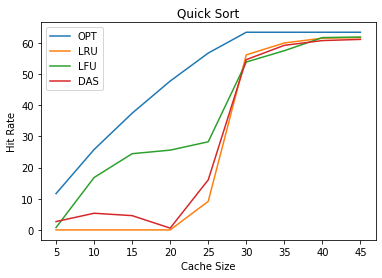
\includegraphics[scale=0.6]{qsort.png}~
       \caption{Quick Sort Trace}\label{Fig:1}
 \end{figure}

 \begin{figure}
        \centering
       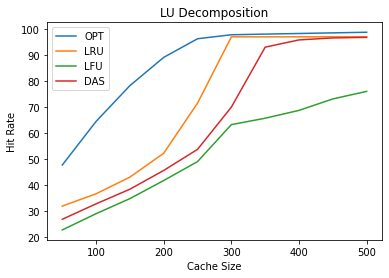
\includegraphics[scale=0.6]{lu.png}~
       \caption{LU Trace}\label{Fig:1}
 \end{figure}

 \begin{figure}
        \centering
       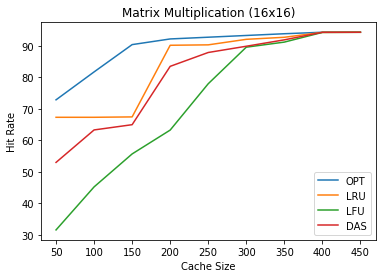
\includegraphics[scale=0.6]{mm16.png}~
       \caption{Matrix Multiplication(16x16) Trace}\label{Fig:1}
 \end{figure}

 \begin{figure}
        \centering
       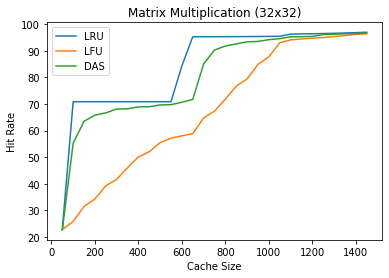
\includegraphics[scale=0.6]{mm32.png}~
       \caption{Matrix Multiplication(32x32) Trace}\label{Fig:1}
 \end{figure}

 \begin{figure}
        \centering
       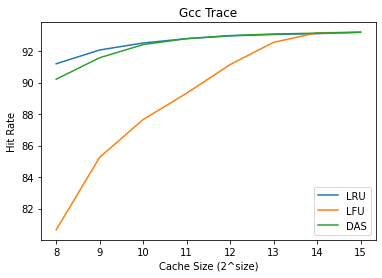
\includegraphics[scale=0.6]{gcc.png}~
       \caption{Gcc Trace}\label{Fig:1}
 \end{figure}

 \begin{figure}
        \centering
       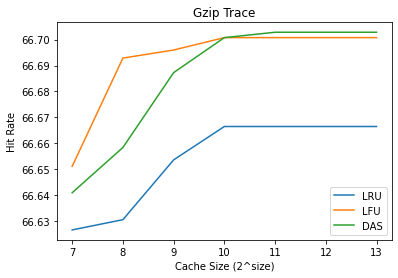
\includegraphics[scale=0.6]{gzip.png}~
       \caption{Gzip Trace}\label{Fig:1}
 \end{figure}

 \begin{figure}
        \centering
       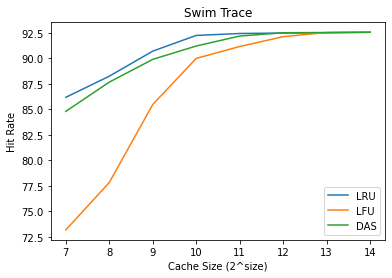
\includegraphics[scale=0.6]{swim.png}~
       \caption{Swim Trace}\label{Fig:1}
 \end{figure}

 \begin{figure}
        \centering
       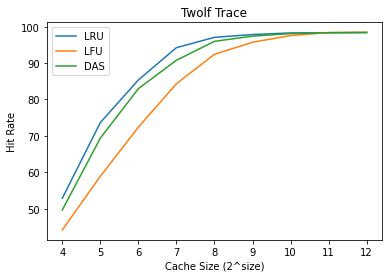
\includegraphics[scale=0.6]{twolf.png}~
       \caption{Twolf Trace}\label{Fig:1}
 \end{figure}

\newpage

\subsection{\textbf{Results of optimal partitioning for all traces}}

We then obtained some more results by comparing different partitions of LRU and LFU portion for DAS policy on those following 8 traces and the results obtained are as follows:

\begin{figure}
        \centering
       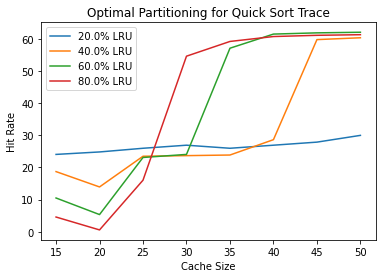
\includegraphics[scale=0.6]{Qsort_partition.png}~
       \caption{Quick Sort Trace}\label{Fig:1}
 \end{figure}

 \begin{figure}
        \centering
       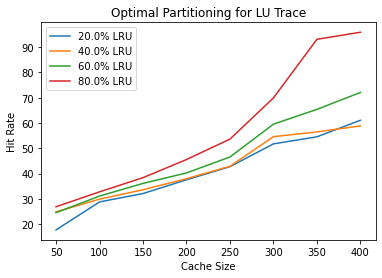
\includegraphics[scale=0.6]{lu_partition.png}~
       \caption{LU Trace}\label{Fig:1}
 \end{figure}

 \begin{figure}
        \centering
       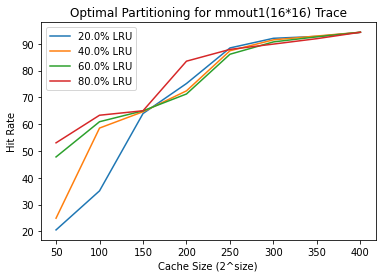
\includegraphics[scale=0.6]{mm16_partition.png}~
       \caption{Matrix Multiplication(16x16) Trace}\label{Fig:1}
 \end{figure}

 \begin{figure}
        \centering
       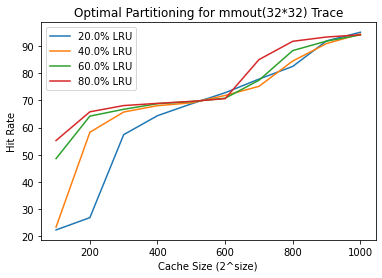
\includegraphics[scale=0.6]{mm32_partition.png}~
       \caption{Matrix Multiplication(32x32) Trace}\label{Fig:1}
 \end{figure}

 \begin{figure}
        \centering
       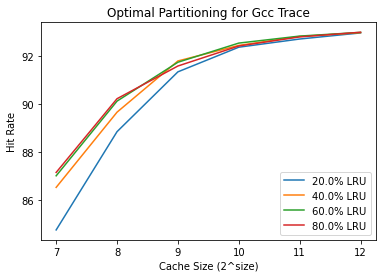
\includegraphics[scale=0.6]{gcc_partition.png}~
       \caption{Gcc Trace}\label{Fig:1}
 \end{figure}

 \begin{figure}
        \centering
       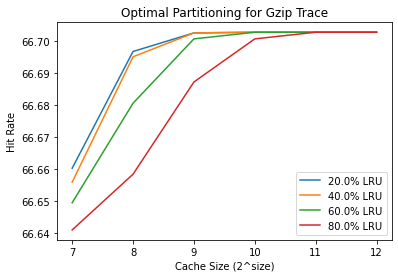
\includegraphics[scale=0.6]{gzip_partition.png}~
       \caption{Gzip Trace}\label{Fig:1}
 \end{figure}

 \begin{figure}
        \centering
       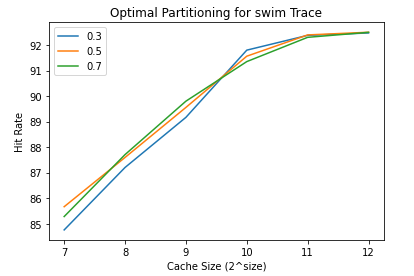
\includegraphics[scale=0.8]{swim_partition.png}~
       \caption{Swim Trace}\label{Fig:1}
 \end{figure}

 \begin{figure}
        \centering
       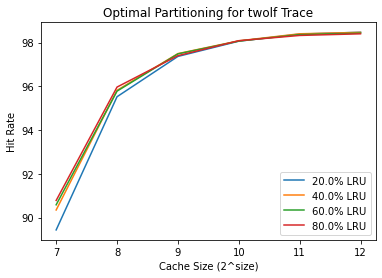
\includegraphics[scale=0.6]{twolf_partition.png}~
       \caption{Twolf Trace}\label{Fig:1}
 \end{figure}
\\

\newpage
\subsection{\textbf{Results for comparison between DAS and Adaptive-DAS}}
Below are the results of comparison of DAS and Adaptive-DAS for those 8 traces:

 \begin{figure}
        \centering
       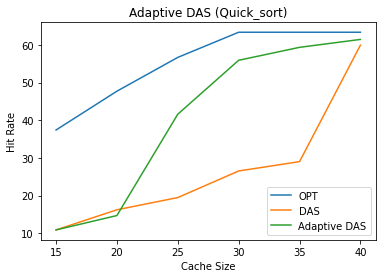
\includegraphics[scale=0.6]{adatpive_qs.png}~
       \caption{Quick Trace}\label{Fig:1}
 \end{figure}

 \begin{figure}
        \centering
       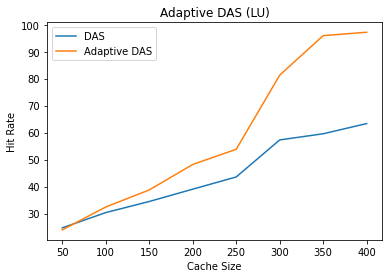
\includegraphics[scale=0.6]{adaptive_lu.png}~
       \caption{LU Trace}\label{Fig:1}
 \end{figure}

 \begin{figure}
        \centering
       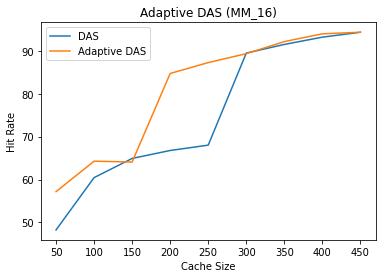
\includegraphics[scale=0.6]{adaptive_mm16.png}~
       \caption{Matrix Multiplication(16x16) Trace}\label{Fig:1}
 \end{figure}

 \begin{figure}
        \centering
       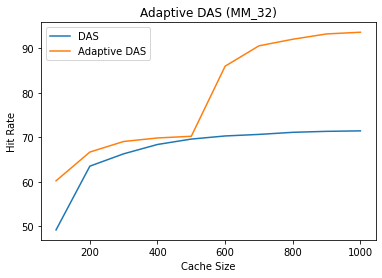
\includegraphics[scale=0.6]{adaptive_mm32.png}~
       \caption{Matrix Multiplication(32x32) Trace}\label{Fig:1}
 \end{figure}

 \begin{figure}
        \centering
       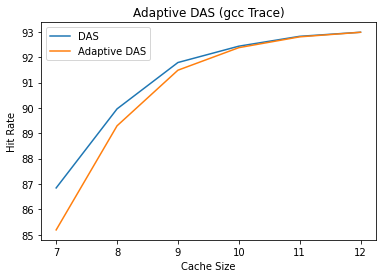
\includegraphics[scale=0.6]{adpative_gcc.png}~
       \caption{Gcc Trace}\label{Fig:1}
 \end{figure}

 \begin{figure}
        \centering
       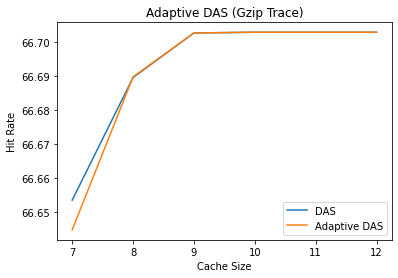
\includegraphics[scale=0.6]{adaptive_gzip.png}~
       \caption{Gzip Trace}\label{Fig:1}
 \end{figure}

 \begin{figure}
        \centering
       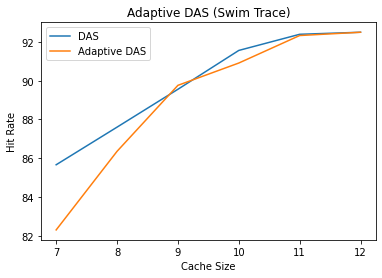
\includegraphics[scale=0.6]{adaptive_swim.png}~
       \caption{Swim Trace}\label{Fig:1}
 \end{figure}

 \begin{figure}
        \centering
       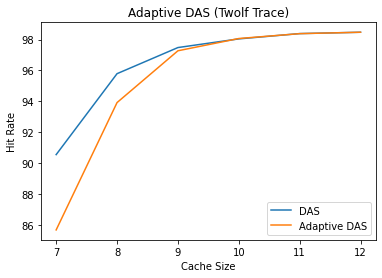
\includegraphics[scale=0.6]{adaptive_twolf.png}~
       \caption{Twolf Trace}\label{Fig:1}
 \end{figure}

\\
\newpage
\section{\textbf{Conclusion}}

From the above results we can see that DAS policy which considers both recency and frequency is sometimes better than LRU and sometimes than LFU. Thus, hybrid cache is better option than only considering recency i.e LRU or frequency i.e LFU.  

Moreover, the adaptive natured cache should be more preferred than just the dynamic one as it brings a major change of adaptivity to the references and thus adapting better to the accesses. The same thing can be seen in the results above. 

\begin{thebibliography}{00}

\bibitem{report1} \href{https://drive.google.com/file/d/1oDsIjIyG2wDHd52hKxKYRgiID0IYgg_g/view?usp=sharing}{DANAPPA-THESIS-2020-(Reference Report)}

\bibitem{r1} \href{http://www.cs.toronto.edu/~reid/csc150/02f/a2/traces.html}{Trace File Resource Link-1}

\bibitem{r2} \href{https://cseweb.ucsd.edu/classes/fa07/cse240a/project1.html}{Trace File Resource Link-2}
\end{thebibliography}


\end{document}
